\begin{frame}[t,plain]
\titlepage
\end{frame}



\begin{frame}[t]{Motivación del proyecto}

\begin{onlyenv}<1>
En el Laboratorio de Electrónica Cuántica (LEC) se dispone de un microscopio SPIM

\begin{columns}
    \begin{column}{0.5\textwidth}
        \begin{itemize}
            \item Utiliza muestras con fluoroforos
            \item Con una hoja de luz (lightsheet) ilumina un plano de la muestra por vez
            \item Disminuye el photobleaching (blanqueo de los flouroforos)
            \item Permite recostruir una imagen en 3D de la muestra
        \end{itemize}
    \end{column}
    \begin{column}{0.5\textwidth}
        \begin{figure}[H]
            \centering
            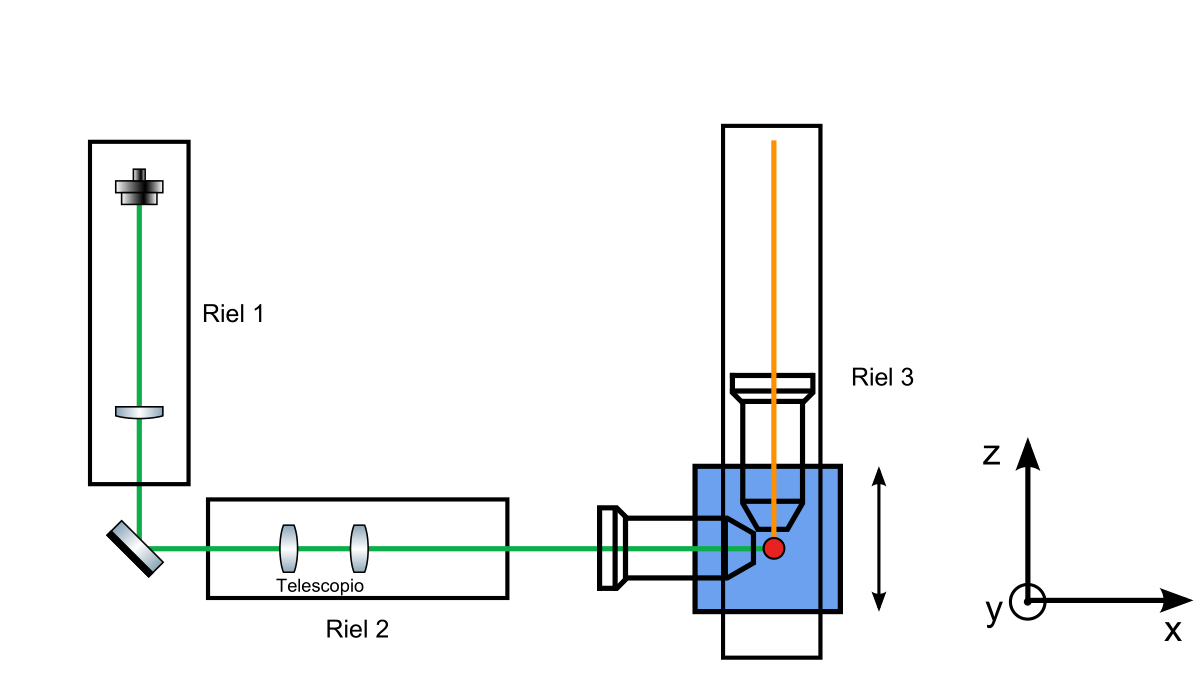
\includegraphics[width=\textwidth]{fig/spim}
            \label{fig:spim} 
        \end{figure}
    \end{column}
\end{columns}
\end{onlyenv}

\begin{onlyenv}<2>
    La construcción de este microscopio requiere determinar
    \begin{itemize}
        \item Perfil del haz, que cambia el tamaño de la hoja del haz
        \item Espectro del haz, determina los flouroforos a utilizar
        \item Polarización del haz, que si es lineal permite hacer mediciones de anisotropía de los fluoroforos
    \end{itemize}
Para determinar esto, se construyó para el siguiente instrumental portátil
\begin{itemize}
    \item Perfilador
    \item Polarimetro
\end{itemize}
\end{onlyenv}

\end{frame}



\subsection{Electronica de adquisición}

\begin{frame}{Electrónica de adquisición}
\begin{columns}[c]
    \begin{column}{0.5\textwidth}
        \begin{itemize}
        \item Considerado un amplificador de corriente. Se mide con amplificador de corriente Standford SR750 y se observa mejoras substanciales
        \item Implementado amplificador de transimpedancia con fotodiodo no polarizado. 
        \item Mejor respuesta en frecuencia y no satura el fotodiodo
        \end{itemize}
    \end{column}
    \begin{column}{0.4\textwidth}
        \begin{figure}[H]
        \centering
        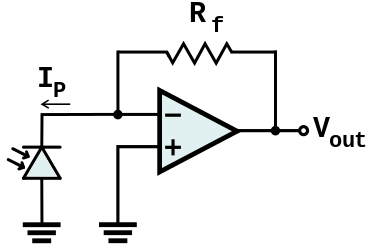
\includegraphics[width=1.1\textwidth]{fig/circuito/amp/TIA.png}
        \label{fig:circuito/amp/TIA}
        \end{figure}
    \end{column}
\end{columns}



\end{frame}

\begin{frame}{Calibración de amplificador}

\begin{columns}[c]
    \begin{column}{0.4\textwidth}
        \begin{itemize}
        \item Amplificador con LM358. Con fuente simple
        \item Respuesta al escalón de 0,4V$\,\mu$s$^{-1}$. 4 veces más grande de la necesaria
        \item Rango lineal bastnate amplio, pero no acusa corriente nula. Se puede buscar otro amplificador. Suficiente para la amplicación
        \end{itemize}
    \end{column}
    %
    \begin{column}{0.5\textwidth}
        \vspace{-1em}
        \begin{figure}[H]
            \centering
            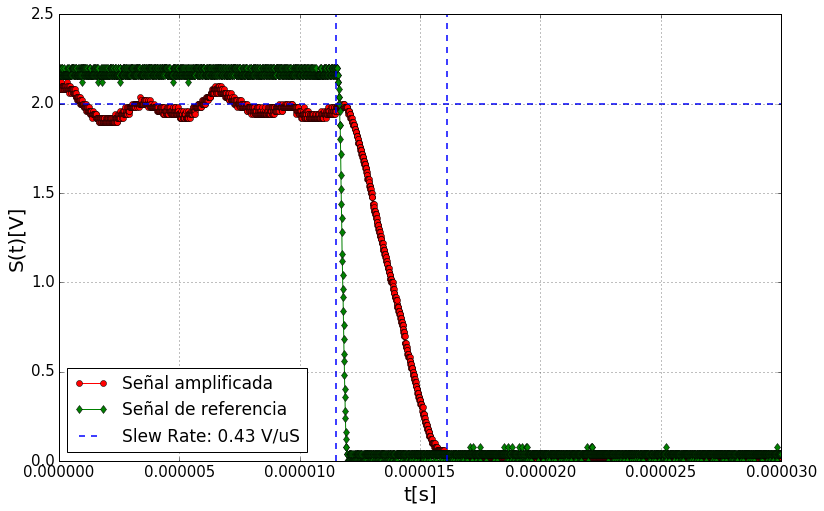
\includegraphics[width=\textwidth]{fig/circuito/amp/transicion_amp}
            \label{fig:transicion_amp}
        \end{figure}
        \vspace{-2em}
        \begin{figure}[H]
            \centering
            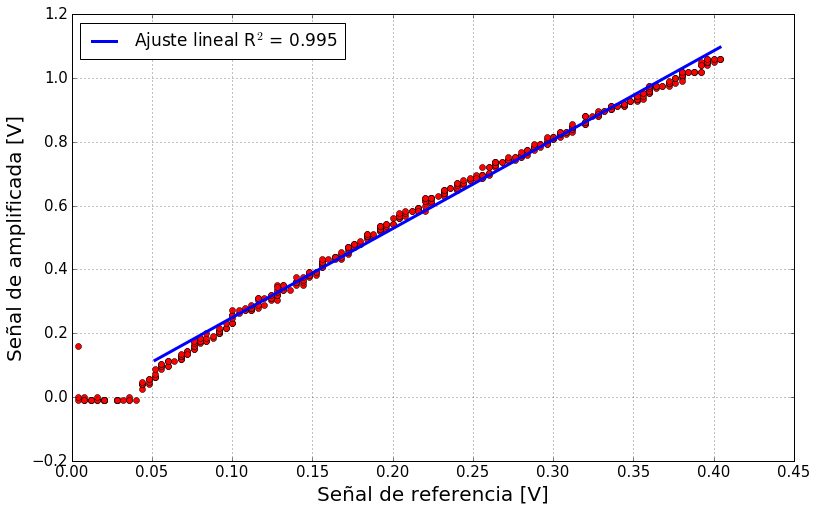
\includegraphics[width=\textwidth]{fig/circuito/amp/lin_amp}
            \label{fig:circuito/amp/lin_amp}
        \end{figure}
    \end{column}
\end{columns}


\end{frame}

\begin{frame}{Generación de sensores portátiles}
\begin{onlyenv}<1>
    \begin{columns}[c]
        \begin{column}{.5\textwidth}
        Spark Photon
        \begin{itemize}
            \item ARM Cortex M3 120MHz con stack WiFi. 
            \item 128KiB RAM y 1MiB FLASH
            \item Programación en la nube, permite actualizaciones OTA.
            \item API de programación más poderosa. C++ por defecto
            \item Software implementado con licencia libre, puede ser adaptado
        \end{itemize}
        \end{column}

        \begin{column}{.2\textwidth}
            \begin{figure}
                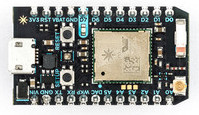
\includegraphics[width=1.7\textwidth]{fig/circuito/photon}
                \label{fig:circuito/photon}
            \end{figure}
        \end{column}
    \end{columns}
\end{onlyenv}

\begin{onlyenv}<2>
    \begin{block}{Resultados con este uC}
        \begin{itemize}
            \item Se pudo mover el motor hasta 30RPS. \\PWM mejor implementado
            \item Adquisición de datos (del uC) cada 10$\mu$s o 100ksps. Más de lo necesario
            \item Conexión TCP ya resuelta, cada 0,1s se obtiene 4000 datos
        \end{itemize}
    \end{block}
\end{onlyenv}

\end{frame}

\subsection{Sofware de adquisción}

\begin{frame}{Software de adquisición}
    \begin{itemize}
        \item Programa efectuado enteramente Python.
        \item Código libre para ser adaptado
        \item Interfaz gráfica, es portable y fácil de instalar
        \item Permite obtener los datos crudos para hacer otros análisis.
        \item Algoritmo de ajuste basado en técnicas de reconocimiento de imágenes
    \end{itemize}
\end{frame}

\subsection{Polarimetro}


\section{Mediciones}


\begin{frame}{Mediciones con el perfilador}

\begin{onlyenv}<1>
Salida de colimador F280FC del SPIM
\begin{columns}[t]
\begin{column}{0.5\textwidth}
    \begin{figure}[H]
    \centering
    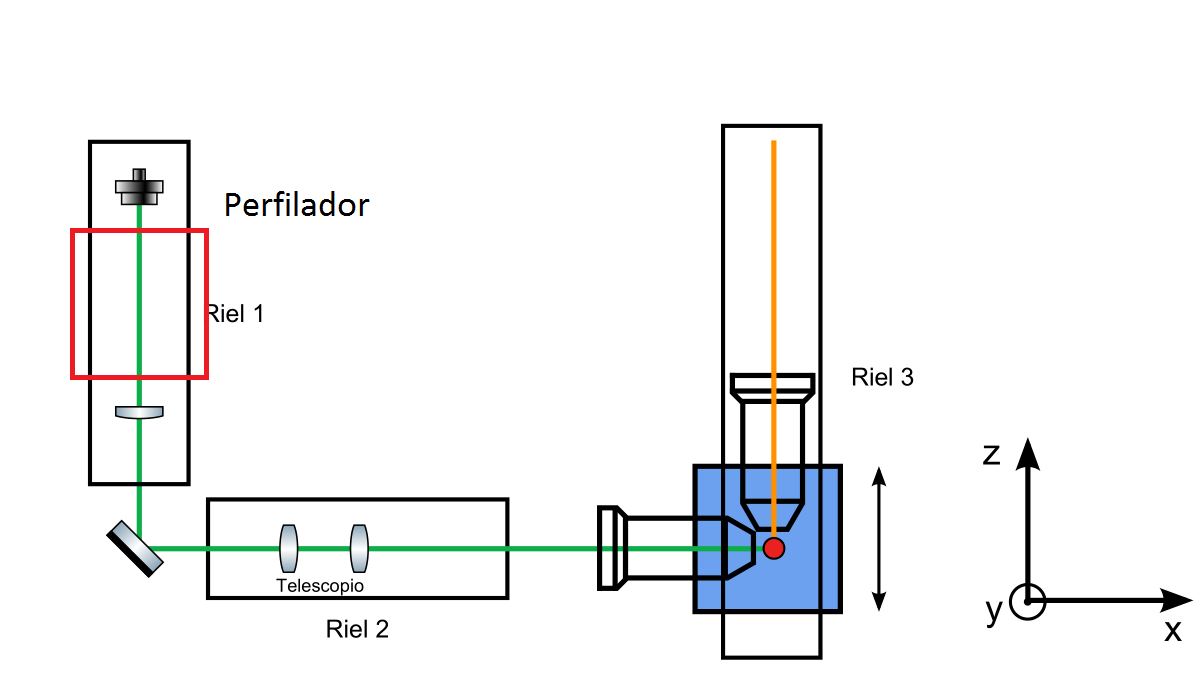
\includegraphics[width=\textwidth]{fig/perfilador/spim_riel_perfilador.png}
    \label{fig:spim_riel_perfilador}
    \end{figure}
\end{column}
%
    \begin{column}{0.5\textwidth}
        \vspace{-2em}
        \begin{figure}[H]
            \centering
            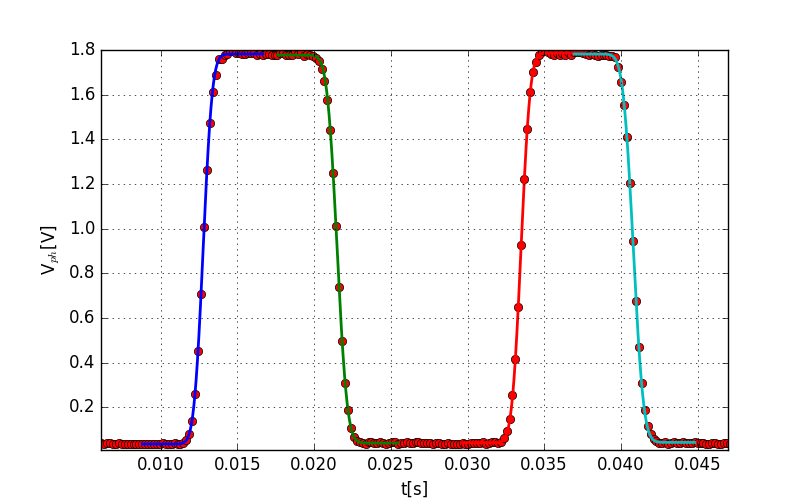
\includegraphics[width=\textwidth]{fig/perfilador/spim_foco_zoom.png}
            \label{fig:spim_foco_zoom}
        \end{figure}
        \vspace{-1em}
        
    
    \end{column}
    
\end{columns}

    \begin{itemize}
            \item Inicio del riel:\\ $\sigma = (3,03 \pm 0,15)\,\text{mm}$
            \item Fin del riel:\\ $\sigma = (3,02 \pm 0,18)\,\text{mm}$
    \end{itemize}
    Colimador \underline{efectivamente colima el haz}
\end{onlyenv}

%\begin{onlyenv}<2>

Haz en el telescopio del SPIM
\begin{columns}[c]
\begin{column}{0.5\textwidth}
    \begin{figure}[H]
        \centering
        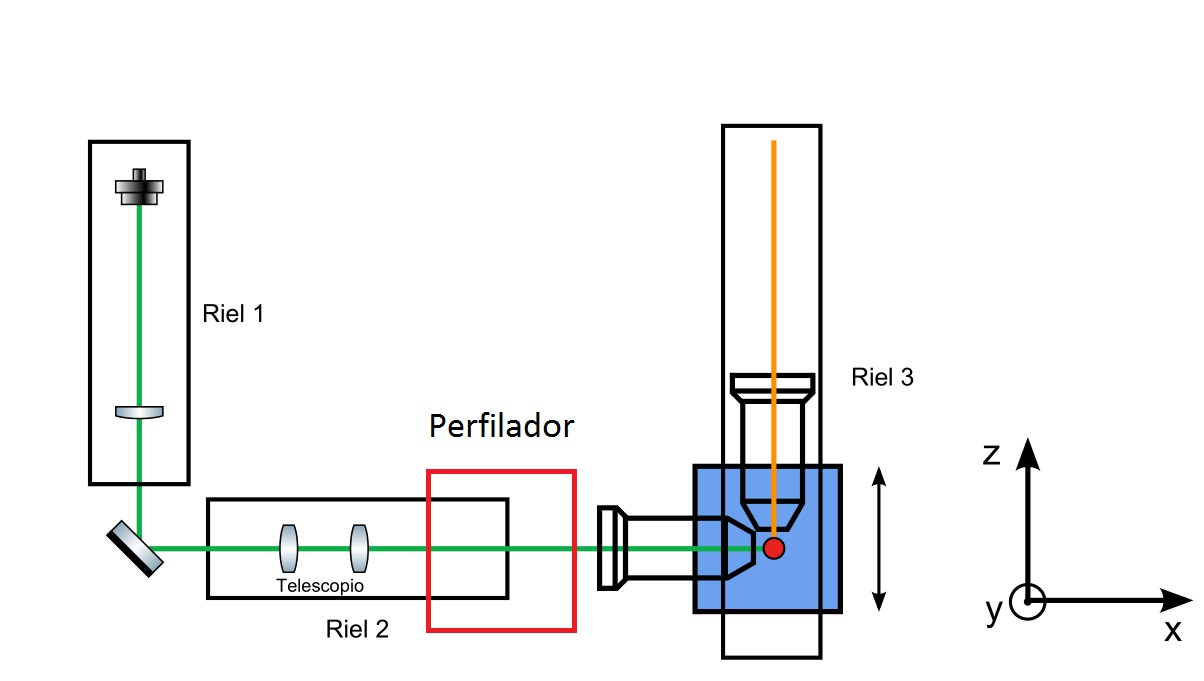
\includegraphics[width=\textwidth]{fig/perfilador/spim_lightsheet_perfilador}
        \label{fig:data_teensy}
    \end{figure}
\end{column}
\begin{column}{0.5\textwidth}
    \vspace{-3em}
    \begin{figure}[H]
        \centering
        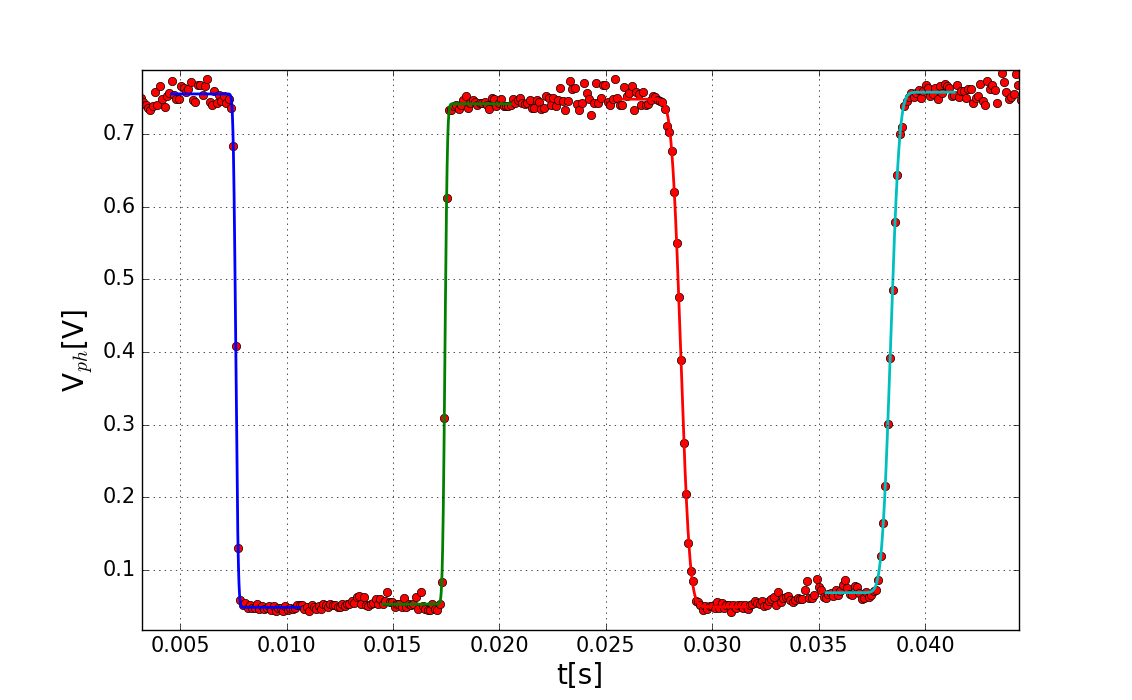
\includegraphics[width=\textwidth]{fig/spim_lightsheet}
        \label{fig:data_teensy}
    \end{figure}
    \vspace{-1em}
    Medición a \\d$\approx$80$\,$mm del fin del telescopio
    $\sigma_1 = (0,55 \pm 0,02)\,\text{mm}$\\
    $\sigma_2 = (2,11 \pm 0,05)\,\text{mm}$\\
    \end{column}
\end{columns}
\vspace{1em}
Las transiciones acusan una \underline{divergencia} apreciable, como es de esperar en un telescopio.

\end{onlyenv}


\begin{onlyenv}<3>
    \begin{block}{Conclusiones de esta medición}
        \begin{itemize}
            \item Se pudo caracterizar el haz dentro del SPIM en todo el trazado
            \item El perfilador fue capaz de medir la divergencia \underline{con solo un set de mediciones}.
            \item El tamaño de la cintura del haz es importante para el microscopio, y tenemos una medición directa fácil de efectuar
        \end{itemize}
    \end{block}
\end{onlyenv}

%\begin{onlyenv}<5>
%Láser Helio Neon 05-LGP-193. $d=80\text{mm}$
%\begin{minipage}[t]{0.5\textwidth}
%\begin{figure}[H]
%\centering
%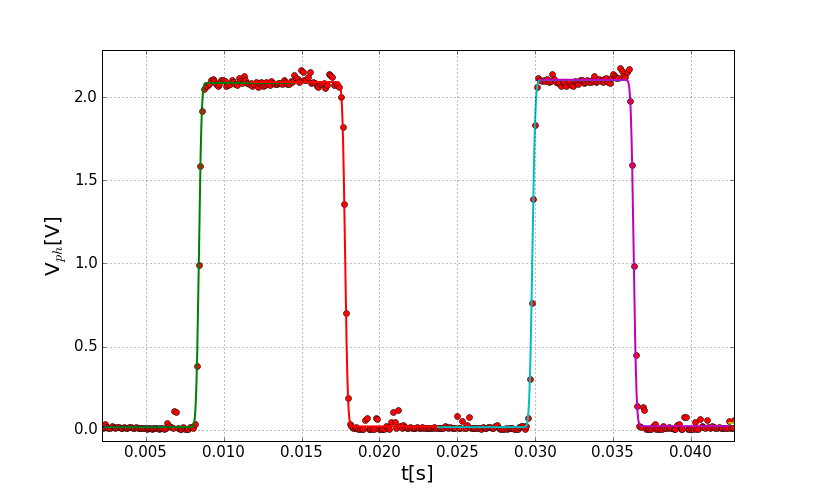
\includegraphics[width=\textwidth]{fig/he_ne_verde_zoom.png}
%\label{fig:data_teensy}
%\end{figure}
%\end{minipage}
%\begin{minipage}[t]{0.46\textwidth}
%\vspace{2em}
%$\sigma = (0,838 \pm 0,20)\,\text{mm}$\\
%Consistente con documentación.
%\end{minipage}
%\end{onlyenv}
\end{frame}






\end{frame}
